\section{含参积分}

\subsection{含参常义积分}

\begin{definition}
	设 $f(x, y)$ 是定义在 $I = [a, b] \times [c, d]$ 上的连续函数，那么若对于任意 $y \in [c, d]$，$f(x, y)$ 关于 $x$ 连续，且积分值 $\int_{a}^{b} f(x, y) \dd{x}$ 由 $y$ 唯一确定，即
	$$
	I(y) = \int_{a}^{b} f(x, y) \dd{x}
	$$
	那么该积分称为\textbf{含参变量 $y$ 的积分}。
\end{definition}

对于一个含有参数 $y$ 的积分式 $I(y) = \int f(x, y) \dd{x}$，我们有一系列定理描述其特性。

首先是连续性：

\begin{theorem}
	设 $f(x, y)$ 是定义在 $I = [a, b] \times [c, d]$ 上的连续函数，那么
	$$
	I(y) = \int_{a}^{b} f(x, y) \dd{x}
	$$
	在 $[c, d]$ 上连续。

	\begin{proof}
		因为 $f(x, y)$ 在闭区域上连续，因此也一致连续。所以
		$$
		\forall\,\varepsilon > 0: \exists\,\delta > 0: \forall\,\vect{x}_1, \vect{x}_2 \in D: \norm{\vect{x}_1 - \vect{x}_2} < \delta \implies \abs{f(\vect{x}_1) - f(\vect{x}_2)} < \varepsilon
		$$
		那么，当 $y - y_0 < \delta$ 时，有
		$$
		\abs{I(y) - I(y_0)} = \abs{\int_{a}^{b} (f(x, y) - f(x, y_0)) \dd{x}} \le \int_{a}^{b} \abs{f(x, y) - f(x, y_0)} \dd{x} \le (b - a) \varepsilon
		$$
		因此 $I(y)$ 在 $[c, d]$ 连续。
	\end{proof}
\end{theorem}

由该定理可知，当 $f(x, y)$ 连续时，极限符号和积分符号可以交换位置：
$$
\lim_{y \to y_0} \int_{a}^{b} f(x, y) \dd{x} = \int_{a}^{b} \lim_{y \to y_0} f(x, y) \dd{x}
$$

然后是可导性：

\begin{theorem}
	设 $f(x, y), f_y(x, y)$ 在 $I = [a, b] \times [c, d]$ 上连续，那么
	$$
	I(y) = \int_a^b f(x, y) \dd{x}
	$$
	在 $[c, d]$ 可导，并且
	$$
	\dv{I}{y} = \int_{a}^{b} f_y(x, y) \dd{x}
	$$
	\begin{proof}
		根据微分中值定理：
		$$
		\begin{aligned}
			\frac{I(y + \Delta y) - I(y)}{\Delta y} & = \int_{a}^{b} \frac{f(x, y + \Delta y) - f(x, y)}{\Delta y} \dd{x} \\
			& = \int_{a}^{b} f_y(x, y + \theta \Delta y) \dd{x}
		\end{aligned}
		$$
		其中 $0 < \theta < 1$。那么可得
		$$
		\dv{I}{y} = \lim_{\Delta y \to 0} \int_{a}^{b} f_y(x, y + \theta \Delta y) \dd{x} = \int_{a}^{b} f_y(x, y) \dd{x}
		$$
	\end{proof}
\end{theorem}

\begin{theorem}
	设 $f(x, y), f_y(x, y)$ 在 $I = [a, b] \times [c, d]$ 上连续，又设 $a(y), b(y)$ 在 $[c, d]$ 可导且 $a \le a(y), b(y) \le b$，那么
	$$
	I(y) = \int_{a(y)}^{b(y)} f(x, y) \dd{x}
	$$
	在 $[c, d]$ 可导，并且
	$$
	\dv{I}{y} = \int_{a(y)}^{b(y)} f_y(x, y) \dd{x} + f(b(y), y) b'(y) - f(a(y), y) a'(y)
	$$
	\begin{proof}
		将 $I(y)$ 看做复合函数，使用复合函数求导即可。
	\end{proof}
\end{theorem}

\subsection{作业}

\begin{problem}
	习题 19.1.1
	\begin{proof}
		\begin{itemize}
			\item 当 $y > 1$ 时：
			$$
			F(y) = \int_{0}^{1} \sgn(x - y) \dd{x} = \int_{0}^{1} (-1) \dd{x} = -1
			$$
			\item 当 $0 \le y \le 1$ 时：
			$$
			F(y) = \int_{0}^{y} \sgn(x - y) \dd{x} + \int_{y}^{1} \sgn(x - y) \dd{x} = \int_{0}^{y} (-1) \dd{x} + \int_{y}^{1} \dd{x} = 1 - 2y
			$$
			\item 当 $y < 0$ 时：
			$$
			F(y) = \int_{0}^{1} \sgn(x - y) \dd{x} = \int_{0}^{1} \dd{x} = 1
			$$
		\end{itemize}
		容易发现 $F(y)$ 在 $(- \infty, + \infty)$ 连续。图像为：

		\begin{figure}[H]
			\centering
			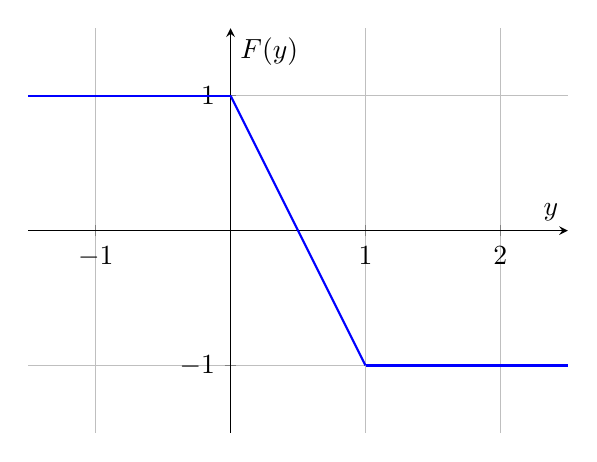
\begin{tikzpicture}
				\begin{axis}[
					axis lines = center,
					axis equal image,
					xlabel = {$y$},
					ylabel = {$F(y)$},
					xmin = -1.5, xmax = 2.5,
					ymin = -1.5, ymax = 1.5,
					xtick distance = 1,
				    ytick distance = 1,
					grid = both,
					important line/.style={thick, blue}
				]
					\addplot[important line, domain=-1.5:0, samples=10] {1};
					\addplot[important line, domain=0:1, samples=10] {1 - 2*x};
					\addplot[important line, domain=1:2.5, samples=10] {-1};
				\end{axis}
			\end{tikzpicture}
			\caption{$F(y) = \int_{0}^{1} f(x, y) \dd{x}$}
		\end{figure}
	\end{proof}
\end{problem}

\begin{problem}
	习题 19.1.2
	\begin{solution}
		\begin{enumerate}
			\item[\textbf{1)}]
			$$
			\begin{aligned}
				\origin & = \int_{-1}^{1} \lim_{\alpha \to 0} \sqrt{x^2 + \alpha^2} \dd{x} \\
				& = \int_{-1}^{1} \abs{x} \dd{x} = 1
			\end{aligned}
			$$
			\item[\textbf{2)}]
			$$
			\begin{aligned}
				\origin & = \int_{0}^{2} \lim_{\alpha \to 0} x^2 \cos \alpha x \dd{x} \\
				& = \int_{0}^{2} x^2 \dd{x} = \frac{8}{3} 
			\end{aligned}
			$$
		\end{enumerate}
	\end{solution}
\end{problem}

\begin{problem}
	习题 19.1.4
	\begin{solution}
		\begin{enumerate}
			\item[\textbf{1)}] 记原积分式为 $I(a, b)$，先假设 $a > 0, b > 0$，那么：
			$$
			\begin{aligned}
				\pdv{I}{a} & = \int_{0}^{\frac{\pi}{2}} \frac{2 a \sin^2 x}{a^2 \sin^2 x + b^2 \cos^2 x} \dd{x} \\
				& = \int_{0}^{\frac{\pi}{2}} \frac{2 a \tan x}{a^2 \tan^2 x + b^2} \dd{x} \\
				& = \int_{0}^{+\infty} \frac{2 a t}{(a^2 t + b^2)(1 + t^2)} \dd{t} \\
				& = \int_{0}^{+\infty} \frac{2a}{a^2 - b^2} \ab(\frac{1}{1 + t^2} - \frac{b^2}{a^2 t^2 + b^2}) \dd{t} \\
				& = \frac{2a}{a^2 - b^2} \ab[\arctan t - \frac{b}{a} \arctan \frac{a t}{b}]_{0}^{+\infty} = \frac{\pi}{a + b}
			\end{aligned}
			$$
			再关于 $a$ 积分回去，得到 $I(a, b) = \pi \ln (a + b) + C(b)$。边界情况：
			$$
			I(b, b) = \pi \ln (2 b) + C(b) = \int_{0}^{\frac{\pi}{2}} \ln (b^2) \dd{x} = \pi \ln b
			$$
			可得 $C(b) = -\pi \ln 2$，最终得到 $I(a, b) = \pi \ln \frac{\abs{a} + \abs{b}}{2}$。

			\item[\textbf{2)}] 设积分式为 $I(a, b)$，那么：
			$$
			\begin{aligned}
				\pdv{I}{a} & = \int_{0}^{\pi} \frac{2 a - 2 \cos x}{1 - 2 a \cos x + a^2} \dd{x} \\
				& = \frac{1}{a} \int_{0}^{\pi} \frac{(1 - 2a \cos x + a^2) + a^2 - 1}{1 - 2a \cos x + a^2} \dd{x} \\
				& = \frac{\pi}{a} + \frac{a^2 - 1}{a} \int_0^\pi \frac{1}{1 + a^2 - 2a \cos x} \dd{x}
			\end{aligned}
			$$
			单独计算这个积分式：
			$$
			\begin{aligned}
				J & = \int_{0}^{\infty} \frac{1}{1 + a^2 - 2a\ab(\frac{1 - t^2}{1 + t^2})} \cdot \frac{2}{1 + t^2} \dd{t} \\
				& = \int_{0}^{\infty} \frac{2}{(1 + a^2) (1 + t^2) - 2a (1 - t^2)} \dd{t} \\
				& = \int_{0}^{\infty} \frac{2}{(1 - a)^2 + (1 + a)^2 t^2} \dd{t} \\
				& = \frac{2}{(1 + a)^2} \int_{0}^{\infty} \frac{1}{t^2 + \ab(\frac{1 - a}{1 + a})^2} \dd{t} \\
				& = \frac{2}{(1 + a)^2} \cdot \frac{\abs{1 + a}}{\abs{1 - a}} \cdot \frac{\pi}{2} = \frac{\pi}{\abs{1 - a^2}}
			\end{aligned}
			$$
			因此 $\pdv{I}{a} = \frac{\pi}{a} + \frac{(a^2 - 1) \pi}{a \abs{1 - a^2}}$。当 $\abs{a} \le 1$ 时，$\pdv{I}{a} = 0$；当 $\abs{a} > 1$ 时，$\pdv{I}{a} = \frac{2\pi}{a}$。积分得到：
			$$
			I(a) = \begin{dcases}
				0 &,\ \abs{a} \le 1 \\
				2 \pi \ln \abs{a} &,\ \abs{a} > 1
			\end{dcases}
			$$
		\end{enumerate}
	\end{solution}
\end{problem}